\title{LA RECONSTITUTION\\ La vèille di gran dz\^{o}}
\author{Administrach\'on comunale de Tsarvensoù}
\date{Tsarvensoù, 2016-2017}

\maketitle

\markboth{\MakeUppercase{\thetitle}}{\MakeUppercase{\thetitle}}

\cleardoublepage 
%\newpage
\vspace*{\fill}
\begin{center}
\textbf{\LARGE Le Digourdì di 2017}
\end{center}

\begin{figure}[h]
\centering
\whiteshadowbox{
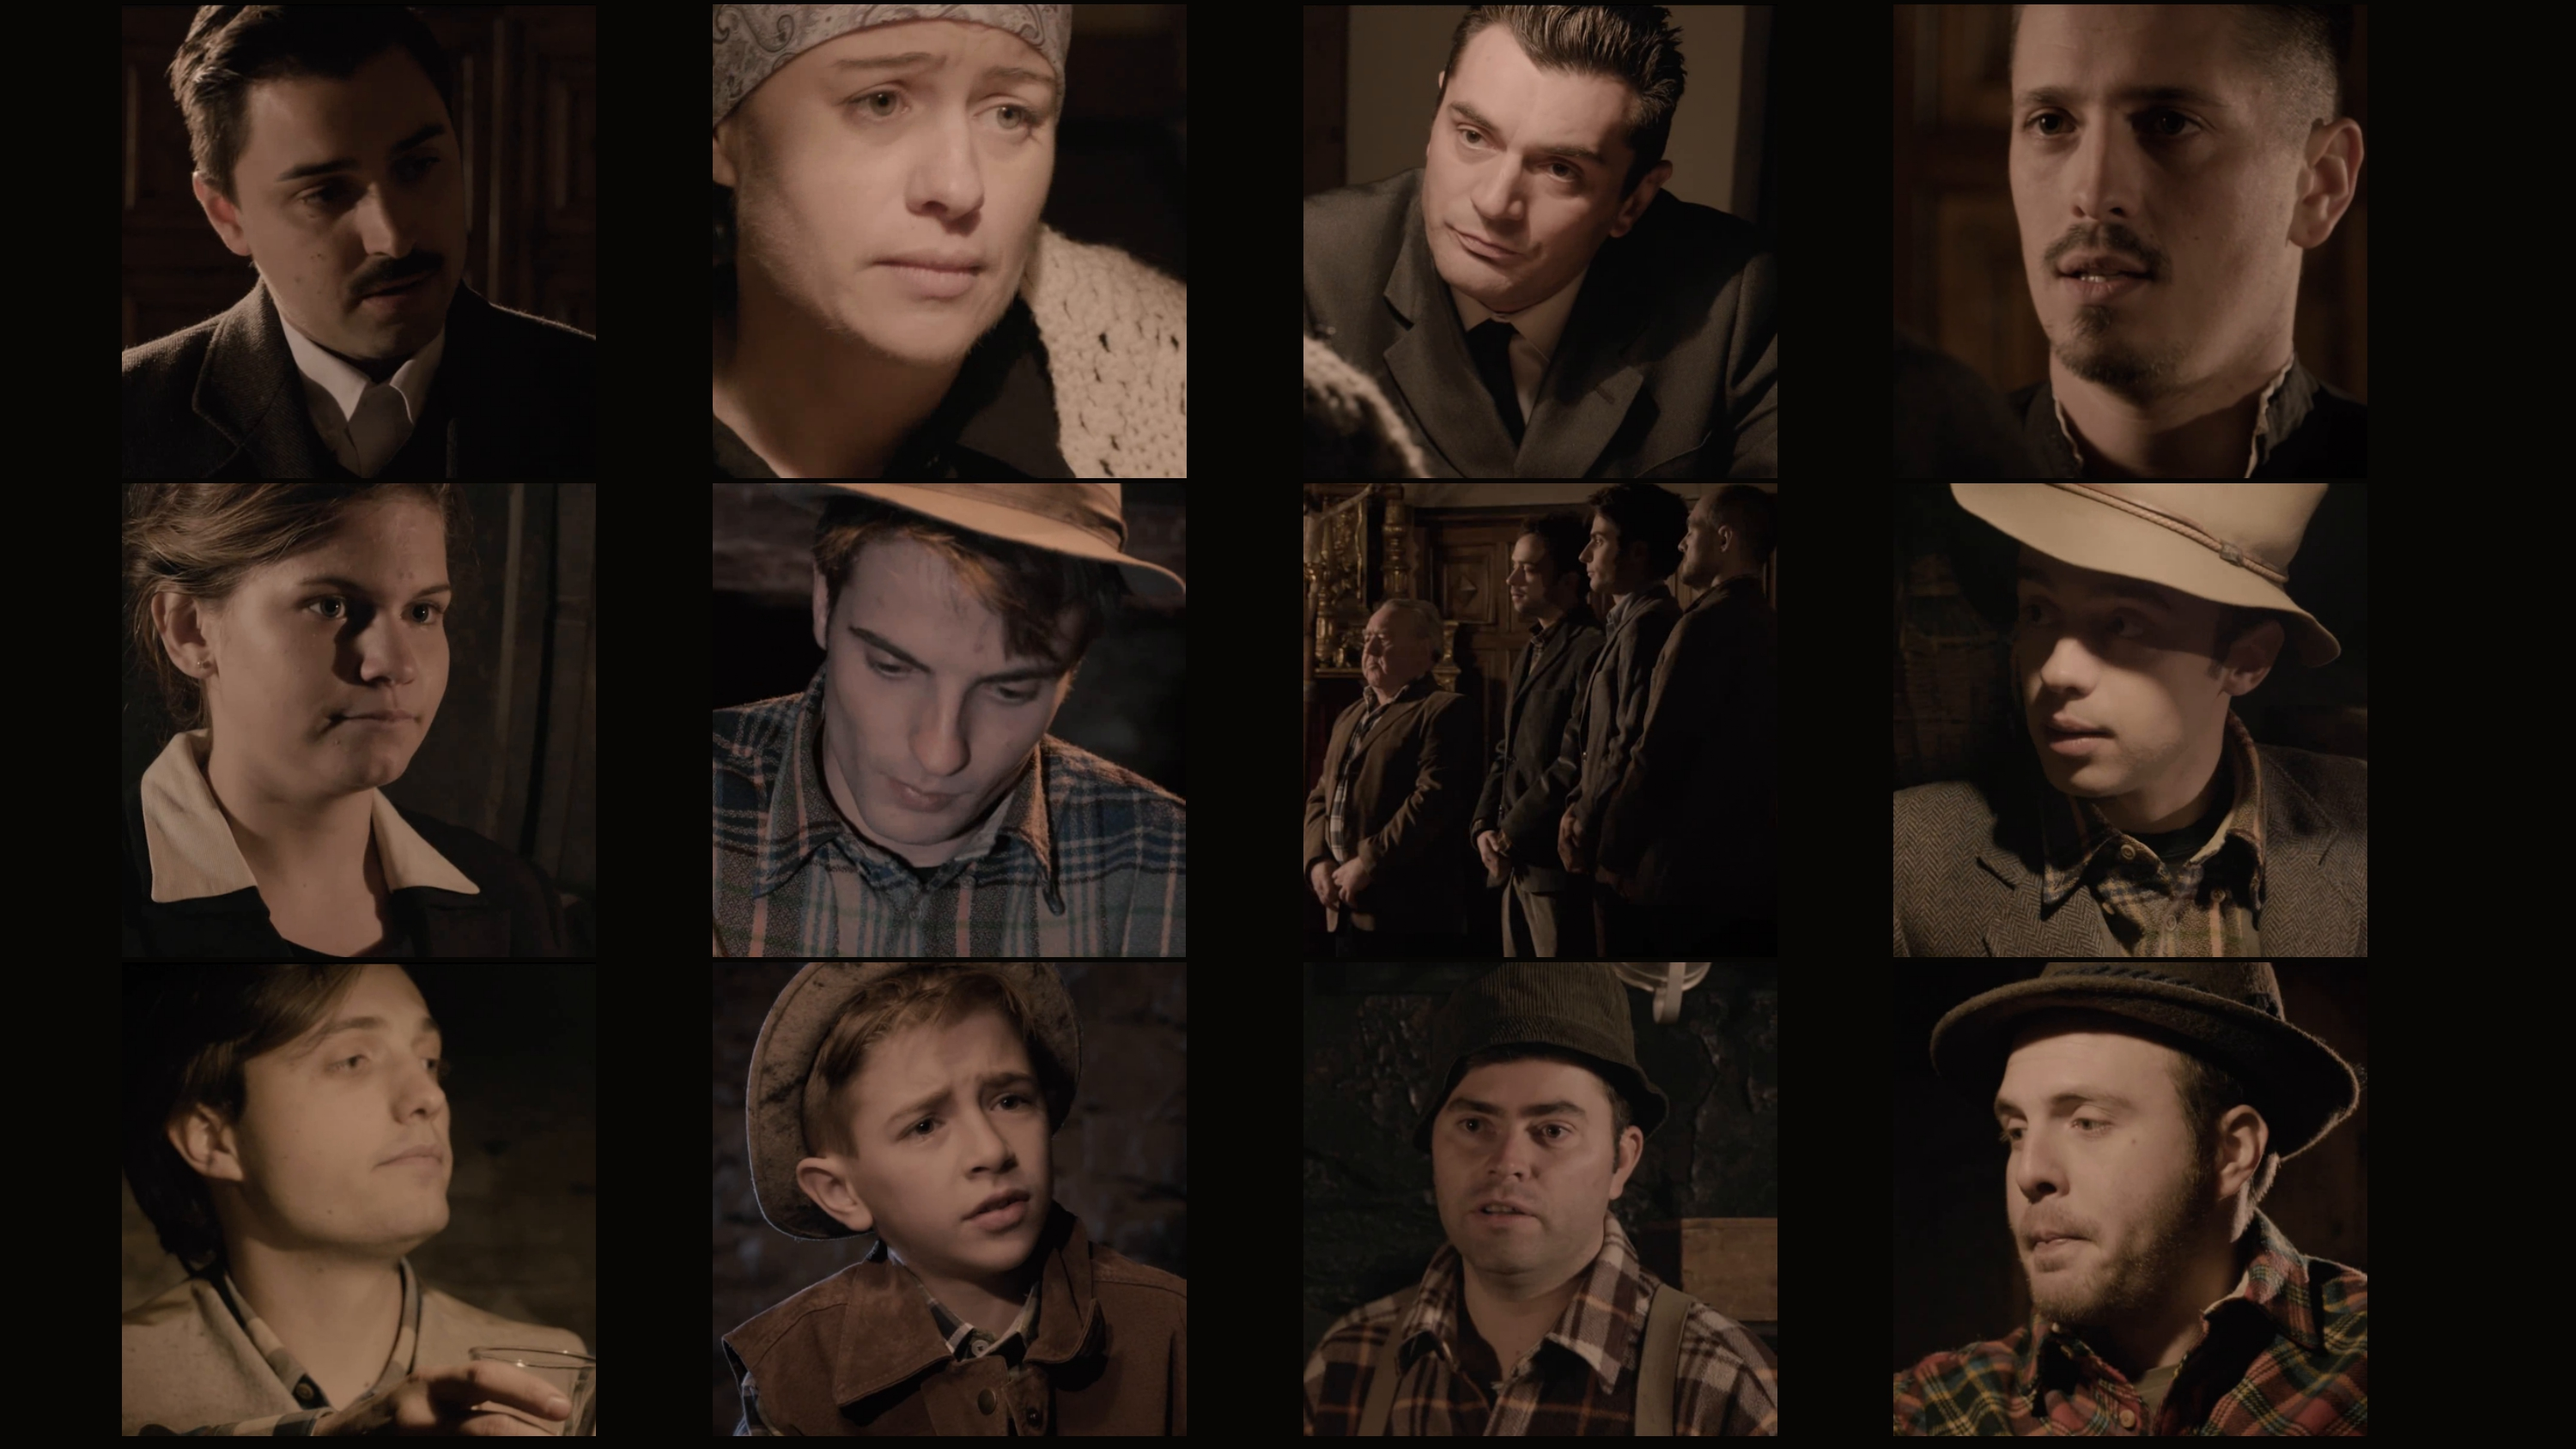
\includegraphics[height=4cm,keepaspectratio]{Foto/2017/gruppo.jpg}
}
\end{figure}
\noindent
\textbf{Dameun}: \textit{Paolo Dall'Ara, Jo\"{e}lle Bollon, Paolo Cima Sander, Marco Ducly.}
\newline
\newline
\textbf{I mentèn}: \textit{Marlène Jorrioz, André Comé, la tsantiì avouì Renzo Bollon, Jordy Bollon,  André Comé é Ronny Borbey, Jordy Bollon.}
\newline
\newline
\textbf{Dézò}: \textit{Richard Cunéaz, Aimé Squinabol, Jo\"{e}l Albaney, Simone Roveyaz.}

\LinkPiese{RECONSTITUTION\\ La vèille di gran dz\^{o}}{https://www.youtube.com/watch?v=A096ZsJ-N0k&t=10s}{.5}

\section*{Eun \textit{court-métrage}?}
Deun l'aout\'on di 2016, l'ie pa eunc\'o cheur que lo Printemps Thé\^atral sarie it\'o organizoù. I mimo ten, le Digourdì l'ayoon resì pe l'Administrach\'on comunale la propozich\'on de réalizé eun courmétradzo avouì eunna équipe de professioniste. L'ie cheur eun projé pa seumplo pe eunna pégna compagnì de téatre sensa espérianse deun lo mondo di \textit{cinéma}. Mi, i mimo ten, l'ie eun projé que l'arie baillà i Digourdì eunna noua voya de recomenchì, aprì eunna dériye pièse, ``N'en pa lo ten", que l'ayè eunna mia tchoué l'entouziasme dedeun la compagnì. 
\\Donque, lo directif l'ayè désidoù de pa partisipé i Printemps Thé\^atral di 2017, deun lo cas que fuche it\'o organizoù\footnote{ \textit{Heuresement} l'è itoù organizoù.}, pe pouèi bouré totte le-z-énerjì deun la produch\'on di premì \textit{court-métrage} di Digourdì.

\section*{Lo souvenir di Seunteucco}
\og N'en voulì counté l'istouére moderne de noutra Quemeua avouì eun langadzo directe, \textit{visuel}, eun proupouzèn i Digourdì eun défì: dzoure leur caletaye é leur espérianse téatrale pe réalizé eun \textit{court-métrage}. Imajin-ì la vèille di premiye-z-éléch\'on tsarvensolentse aprì la Secounda Guerà mondiale, l'a bailla-no la possibilitoù de rappelé tcheu sise que l'an i a queur Tsarvensoù, mimo aprì le-z-àn teuppe di \textit{fascisme}; mi surtoù de commémoré le sinque Père de Tsarvensoù (comme lamo le querì mé!), que l'an portoù la Quemeua i premiye-z-éléch\'on de Tsarvensoù reconstituite.
\\Personellamente, l'è it\'o émouvàn veure comme se pou baillì viya a eun boc\'on d'istouére avouì l'\textit{art cinématographique}. Mimo lo fé que le-z-atteur sayoon de dzouveun-o Tsarvensolèn l'è eun souvenir prèsieu que n'i\ldots pequé, eunsemblo, n'en cougnì, é eun caque magniye viquì, eunna padze eumpourtanta de noutra Communoté.
%Anche il fatto che gli attori fossero tutti giovani e del territorio ha permesso che anche loro venissero a conoscenza di una pagina che ignoravano.
%Personalmente, è stato emozionante veder ricostruire all'interno di un set cinematograrica la storia del nostro comune
%Perché abbiamo voluto raccontare la storia moderna del nostro comune utilizzando un linguaggio immediato e proponendo ai diogurdì una sfida, ossia di cimentarsi nella realizzazione di una pièce teatrale.
%Ripercorre la storia della notte prima delle elezioni, ci ha permesso di ricrodare tutti coloro chehanno sempre avuoto a cuore il nostro comune nonostante gli anni bui della sopressione e soprattutto i cinque,c he amo def padri fondagori, che in prima persona hanno portato il comune alle libere elezioni del 46 continuando per la maggior parte l'impegno nella legislatura successiva.
\fg{}
\newline
\newline
\hspace*{\fill} \textit{Ronny Borbey}

%

\queriaouzitou{
\begin{itemize}
\item[$\bullet$]  \og La vèille di grand dz\^o \fg{} l'è it\'o lo premì \textit{court-métrage} de la compagnì Le Digourdì.\vfill

\item[$\bullet$] \og La vèille di grand dz\^o \fg{} l'è eunc\'o lo débù de Aimé Squinabol deun Le Digourdì comme acteur. L'ie dza pouyà si lo palque deun l'an 2012, mi maque avouì eunna pégna apparich\'on sensa battiye.\vfill

\item[$\bullet$] Renzo, que eunterprète eun tsantre de la parotse, sayè pa qué que sarè itoù reprèi. Jordy l'ayè maque deu-lei que dèijè baillì eunna man pe tramé de moublo.
\end{itemize}
}

\Scenographie
\begin{itemize}
\item[$\bullet$] \'Eillize de \textit{Sainte Colombe} - Tsarvensoù;
\item[$\bullet$] Lèitì di veladzo di Plan - Euntroù;
\item[$\bullet$] \textit{Maison} Bruil d'Euntroù - Crotta avouì 1 tabla, 3 caèye, 1 botéill\'on, 3 vèyo é eunna bocon-où;
\item[$\bullet$] Pailleu avouì 1 banquetta;
\item[$\bullet$] 1 tsaèn avouì de boate;
\item[$\bullet$] \textit{Centre d'études francoprovençales} René Willien - Quezeun-a di-z-àn '40 avouì 1 tabla é 2 caèye. 
\end{itemize}

\setlength{\lengthchar}{3.40cm}

\Character[EMERICO]{}{g}{Emerico Comé, Tsarvensolèn classe 1890, directeur de la tsantiì deun le-z-àn '40, \name{Paolo Dall'Ara}}

\Character[Tsantre I]{}{g}{Tsantre de la parotse de Tsarvensoù, \name{Jordy Bollon}}

\Character[Tsantre II]{}{g}{Tsantre de la parotse de Tsarvensoù, \name{Renzo Bollon}}

\Character[Tsantre III]{}{g}{Tsantre de la parotse de Tsarvensoù, \name{Ronny Borbey}}

\Character[Tsantre IV]{}{g}{Tsantre de la parotse de Tsarvensoù, \name{André Comé}}

\Character[PRIYE]{}{g}{Abbé Hilarion Vection, priye de Tsarvensoù, \name{Marco Ducly}}

\Character[LOUIS]{}{g}{Louis Lucianaz, Tsarvensolèn classe 1901, \name{Jo\"{e}l Albaney}}

\Character[ADELLINE]{}{g}{Adelline Lucianaz, métressa de l'icoula de Tsarvensoù deun le-z-àn '40, \nameF{Marlène Jorrioz}}

\Character[AMÌ DE AIMÉ I]{}{g}{Eun Tsarvensolèn que lame djouì a la moura, \name{Richard Cunéaz}}

\Character[AMÌ DE AIMÉ II]{}{g}{Eun Tsarvensolèn que lame djouì a la moura, \name{Simone Roveyaz}}

\Character[AIMÉ]{}{g}{Aimé Damien Borbey, Tsarvensolèn classe 1897, \name{Jordy Bollon}}

\Character[JOSEPH]{}{g}{Mèinoù tsarvensolèn di-z-àn '40, \name{Aimé Squinabol}}

\Character[JUSTIN]{}{g}{Justin Donzel, Tsarvensolèn classe 1898, \name{André Comé}}

\Character[SABINE]{}{g}{Sabine Lucianaz Savioz, fenna de César Savioz, \nameF{Jo\"{e}lle Bollon}}

\Character[C\'ESAR ]{}{g}{César Savioz, Tsarvensolèn classe 1897,  \name{Paolo Cima Sander}}

\DramPer

\act[RECONSTITUTION\\ La vèille di gran dz\^{o}]

Aprì la Secounda Guèra mondiale, lo 17 di mèis de mi di 1945, lo préfé de Veulla Alessandro Passerin d'Entrèves publiye eunna \textit{circulaire} pe la reconstituch\'on de totte le Quemeue rantchaye pe lo réjime fasiste.

Lo 27 janvieur 1946, 424 Tsarvensolèn é Tsarvensolentse dimandon a la Préfetteua de Veulla la reconstituch\'on de la Quemeua de Tsarvensoù. Lo 30 avrì 1946, lo prof. Federico Chabod, Prézidàn di Conseille de la Val d'Outa, décllare la reconstituch\'on de Tsarvensoù.

Lo 30 joueun 1946, son élì sinque \textit{membre} de la jeunte euntsardjaye de refondé la Quemeua: Aimé Borbey, Emerico Comé, Justin Donzel, Louis Lucianaz é César Savioz.

Lo 23 novembre 1946, vèille di premiye-z-éléch\'on comunale de Tsarvensoù reconstituiya, Aimé, Emerico, Justin, Louis é César viquèison Tsarvensoù comme totte le-z-atre nite, mi avouì lo queur que  boueuche i dzor aprì, lo gran dzor. Eunna nite coloraye avouì salle attivitoù jénuine d'eunna pégna communoté: le proue de la tsantiì, la lèitì, le counte avouì le-z-amì, le traille de la véillà, la chaleur de la fameuille. Eunna nite icllériaye di fouà de la spéranse que brille deun le joueu  queriaou di pégno Joseph. Demàn se recomenche, \textit{démocratiquement}, avouì eun Consèille tsarvensolèn.

\DeriLeRido
\RoleNoms{Sujé é teste}{Le Digourdì,
Chiara Bernardi, Ronny Borbey}
\RoleNoms{Traduch\'on}{Raffaella Lucianaz}
\RoleNoms{Son}{Giovanni Corona, Raffaele D'Anello}
\RoleNoms{Produch\'on ézécutive}{Giulia Di Francescantonio}
\RoleNoms{Produch\'on}{\textit{Ezechiele} 25$:$17}
\RoleNoms{Fotografie é réjì}{Alessandro Stevanon}